\documentclass[runningheads]{llncs}

\usepackage[T1]{fontenc}
\usepackage[utf8]{inputenc}
\usepackage{graphicx}
\usepackage{lettrine}

\begin{document}

\title{Visualization of Single-Cell Transcriptomics from Zebrafish Pigment Cells}
\titlerunning{Visualization of Single-Cell Transcriptomics from Zebrafish Pigment Cells}

\author{Diogo Esteves\inst{1}\orcidID{0000-0001-5741-5686} \& David Henriques\inst{2}\orcidID{0000-0002-9477-292X}}
\authorrunning{D. Esteves \& D. Henriques}

\institute{
    Department of Informatics, University of Minho, Portugal \\
    \email{pg28935@uminho.pt} \and
    CSIC IIM, Vigo, Spain \\
    \email{davidh@iim.csic.es}
}

\maketitle

\begin{abstract}
Zebrafish (\textit{Danio rerio}) represent an essential model organism for studying the mechanisms of disease and vertebrate development. Their unique coloring patterns offer special insights into genetic control and cellular differentiation. In order to investigate the complexity of pigment cell development in zebrafish, this work uses single-cell transcriptomics, which provides hitherto unheard-of precision into the dynamics of cellular heterogeneity and gene expression. By utilizing state-of-the-art tools like scRNA-seq and sophisticated analytical techniques like UMAP and t-SNE, we want to clarify the processes involved in pigment cell development while emphasizing the function of transcription factors and genetic networks. Our work intends to provide a deeper understanding of the genetic origins of pigmentation, which could have far-reaching ramifications for biomedicine, in addition to filling important knowledge gaps in developmental biology. This comprehensive approach is required for the investigation of genetic variation and cellular development inside this well researched model organism.
\end{abstract}

\section{Introduction}
\lettrine[]{S}{}tudying the pigmentation of \textit{D. rerio} cells offers valuable insights into genetic and developmental processes, in addition to being aesthetically pleasing. \textit{D. rerio} is a crucial model organism in biology, understanding its genetic regulation and cellular differentiation can be inferred visually from their distinct pigmentation patterns, which are controlled by various types of pigment cells. As recent research has shown \cite{subkhankulova2023zebrafish,howard2021atlas}, these patterns originate from a highly multipotent progenitor. Although single-cell transcriptomics offers a detailed view of cellular heterogeneity and gene expression dynamics, conventional bulk mRNA sequencing techniques fail in capturing the cellular complexity and dynamic nature of living tissues \cite{nayak2021hitchhiker}.

A recent technique, called single-cell transcriptomics, makes it possible to examine gene expression at the individual cell level, revealing the variety and dynamics of cellular states \cite{nayak2021hitchhiker}. According to Saunders \textit{et al}. \cite{saunders2023embryo}, this method is crucial for tracking the lineage and differentiation pathways of pigment cells in \textit{D. rerio}, offering previously unseen clarity \cite{howard2021atlas}.

\section{State of the Art}
Sur \textit{et al}. (2023)'s study provides a detailed analysis of shared signatures and transcriptional diversity during the development of \textit{Danio rerio}, highlighting the complexity of cell development trajectories captured by advanced technology of single cell transcriptomy \cite{sur2023single}. These findings are parallel to those observed in studies on sensory nodes in vertebrates, where Vermeiren \textit{et al}. (2020) discussed how transcription programs can direct functional specialization, suggesting similar underlying genetic mechanisms that may be in play in the differentiation of pigment cells in zebrafish \cite{vermeiren2020vertebrate}.

\subsection{Single Cell Transcriptomics}
With the rapid advancement of single-cell transcriptomics, which provides insights into cellular heterogeneity and gene expression patterns within organisms, the field has gone from being an innovative technique to an essential part of contemporary biological research. Novel approaches that have deepened our understanding of cellular processes have fueled this advancement \cite{kulkarni2019beyond}.

\subsection{Advancements in Single-cell Technologies}
Thanks to technological developments like the 10x Genomics Chromium system, which have enabled thorough molecular profiling at high throughput, zebrafish pigmentation and the underlying genetics have progressed \cite{srivatsan2020massively}. In a short period of time, single-cell transcriptomics has evolved from a novel technique to a standard in biological research. This technique has made it possible to thoroughly examine gene expression at the level of individual cells, giving previously unachievable insights into the heterogeneity of cells within organisms. 

Innovations such as Drop-seq and the 10x Genomics Chromium system have been essential in opening a window into the cellular heterogeneity and transcriptional landscapes of developing organisms \cite{nayak2021hitchhiker}. These advancements have been essential in deciphering the complex mechanisms behind zebrafish pigmentation and have improved our understanding of the effects of both genetics and environment on pigment cell differentiation \cite{qiu2017reversed}.

\subsection{Analytical Methodologies}
The proliferation of single-cell data has necessitated the development of advanced analytical methods to interpret the complex datasets generated by scRNA-seq. Dimensionality reduction techniques like t-SNE and UMAP are now essential for reducing high-dimensional data into a form that can be understood in order to help identify different cell populations and states \cite{kulkarni2019beyond,nayak2021hitchhiker}.

These techniques facilitate the identification and distinction of various cell populations and states in a variety of sample kinds. Because UMAP can handle larger datasets without compromising the data's global structure, it is especially well-suited for integrating datasets under a variety of experimental conditions. However, careful parameter selection and data preprocessing are required to yield meaningful insights \cite{nayak2021hitchhiker}.
\begin{figure}[htbp]
    \centering
    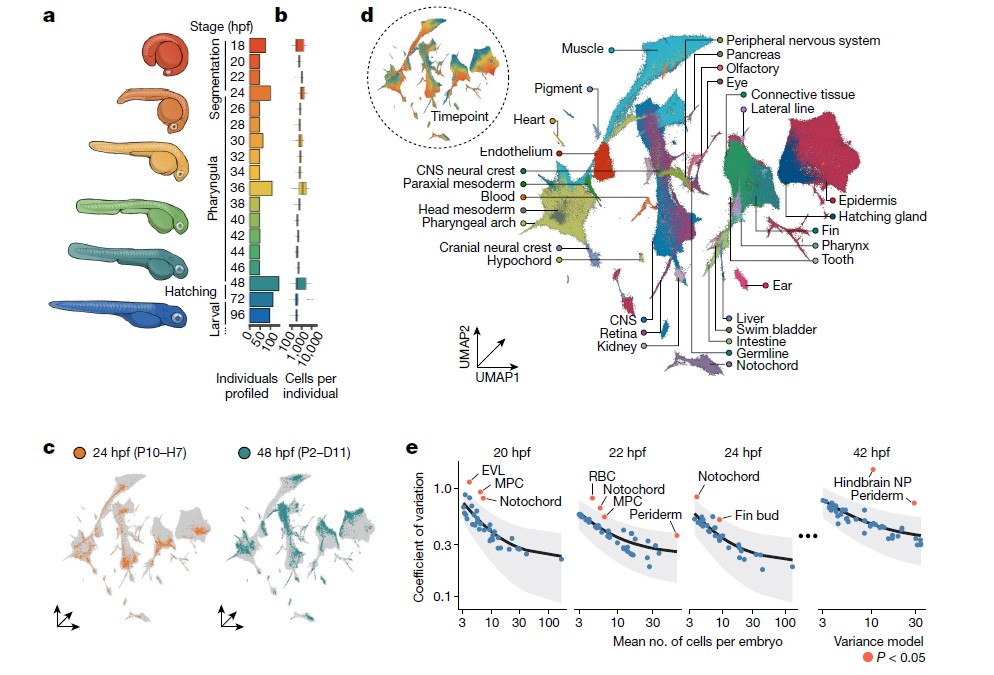
\includegraphics[width=\textwidth]{Fig1.jpg}
    \caption{(a) Development stages of zebrafish from segmentation to larval stages with hours post-fertilization (hpf). (b) Number of cells profiled per individual at each stage. (c) UMAP projections at 24 hpf and 48 hpf showing developmental cell transitions. (d) UMAP visualization highlighting the diversity of cell types and their developmental pathways. (e) Analysis of cell type variance at different developmental timepoints, illustrating the dynamics of cell type distribution. Image adapted from Saunders \textit{et al}., 2023 \cite{saunders2023embryo}.}
    \label{fig:development_stages_cells}
\end{figure}
Moreover, the comprehensive integration of single-cell data, as discussed by Stuart \textit{et al}. \cite{stuart2019comprehensive}, highlights the importance of merging various data sources and types to enhance the understanding of complex biological systems. This integration is important for the advance in our ability to decipher the multifaceted nature of genetic regulation and cellular behavior in development. Stuart \textit{et al}. emphasize the utility of combining single-cell transcriptomics data with other data types to provide a more holistic view of cellular functions and states, which is crucial for our analysis of zebrafish pigmentation patterns.

We will use tools like Slingshot and Monocle, as well as cutting-edge dimensionality reduction techniques and pseudo-time analysis, to achieve our objectives \cite{qiu2017reversed,street2018slingshot}. We will be able to trace the developmental trajectories of pigment cells by methodically arranging cells according to their similarity thanks to these methodologies \cite{nayak2021hitchhiker,kulkarni2019beyond}.

\section{Objective}
This study's main goal is to close the knowledge gaps about the dynamics of gene expression during pigment cell development in \textit{D. rerio} and cellular heterogeneity. By doing this, we hope to clarify the processes underlying pigment cell development and identify the regulatory systems at play.

In addition to exploring cellular differentiation trajectories, a critical objective of this study is to investigate the dynamics of transcription factors during these processes. Kenny \textit{et al}. (2022) show that TFAP2 paralogs facilitate access to chromatin for MITF in pigmentation and cell proliferation genes, highlighting the significant role of these factors in gene expression modulation during pigment cell differentiation. 

These findings underline the importance of analyzing the function of transcription factors in the development of pigment cells in \textit{Danio rerio}.

\subsection{Visualize Cellular Differentiation Trajectories}
We intend to use computational tools like UMAP and t-SNE in conjunction with trajectory inference techniques like Monocle \cite{qiu2017reversed} to visualize and analyze the cellular differentiation trajectories leading to pigment cell development in \textit{D. rerio}. This will enable us to distinguish between different cellular states and transitions during the differentiation process, thereby revealing the intricate regulatory mechanisms driving pigment cell formation.

We will use tools like Slingshot \cite{street2018slingshot} and Monocle, along with cutting-edge dimensionality reduction techniques and pseudo-time analysis, to accomplish our goals. With the help of these techniques, we will be able to map out the developmental paths of pigment cells by methodically arranging cells according to how similar they are. 

Our goal is to further our understanding of the mechanisms regulating zebrafish pigmentation by identifying cell-type lineages and highlighting important gene markers indicative of pigment cell differentiation through the use of these cutting-edge bioinformatics tools.

\subsection{Extract Information on Transcription Factor Dynamics}
Our objective is to examine and describe the modifications in the expression of transcription factors (TF) along the recognized cellular developmental pathways. Finding the important transcription factors (TFs) that control pigment cell differentiation will provide insights into the genetic networks governing this developmental process \cite{subkhankulova2023zebrafish,saunders2019thyroid,fabian2022lifelong}. 

With potential applications in disease treatment, cosmetic research, and environmentally friendly aquaculture practices, these findings may open the door for novel genetic interventions that manipulate pigment cell formation and function.

\section{Tasks}

\subsection{Visualization of Cellular Differentiation Trajectories}
High-throughput single-cell RNA sequencing will be used to investigate pigment cell development in detail, with an emphasis on identifying important transcription factors and genes involved in cell differentiation \cite{srivatsan2020massively,kulkarni2019beyond}:
    \begin{itemize}
        \item \textbf{Single-Cell RNA Sequencing}
        Our goal is to produce a foundational dataset that outlines each cell's transcriptional landscape as it differentiates into \textit{D. rerio} pigment cells. Using high-throughput single-cell RNA sequencing technologies, \textit{D. rerio} samples from different embryonic stages are processed, with a focus on tissues rich in pigment \cite{srivatsan2020massively}.
        \paragraph{}
        \item \textbf{Dimensionality Reduction and Clustering}
        We will use dimensionality reduction methods like UMAP and t-SNE on the scRNA-seq data in order to identify different cell populations and states within the intricate dataset. Indicative of similar biological states or functions, this will assist in identifying cell populations \cite{kulkarni2019beyond,nayak2021hitchhiker}.
        \paragraph{}
        \item \textbf{Trajectory Inference Analysis}
        We intend to map pigment cell developmental trajectories, following their lineage from progenitors to mature states, using trajectory inference tools such as Monocle. This will allow us to identify regulatory genes and important transition states involved in pigment cell development, as well as analyze the temporal progression of cells along differentiation pathways \cite{qiu2017reversed}.        
    \end{itemize}
    
\subsection{Transcription Factor Dynamics}
In order to analyze the temporal progression of cells along differentiation pathways and identify important transition states and regulatory genes involved in pigment cell development, we will use trajectory inference tools like Monocle \cite{qiu2017reversed}.

    \begin{itemize}
        \item \textbf{Differential Expression Analysis}
        To find TFs and genes that are differentially expressed, we will carry out differential expression analysis both across cell clusters and along inferred trajectories. The results of this analysis will identify potential players in the regulation of pigment cell differentiation. Utilizing software intended for RNA-seq data analysis on a single cell, we will employ computational packages \cite{nayak2021hitchhiker,kulkarni2019beyond}.        
        \paragraph{}
        \item \textbf{Validation of Key Transcription Factors}
        We will use in situ hybridization and immunocytochemistry techniques to validate the spatial and temporal expression patterns of important TFs in \textit{D. rerio} tissue sections in order to confirm the role of identified TFs in pigment cell differentiation. This stage establishes the study's empirical foundation by guaranteeing that the computational predictions faithfully capture biological reality \cite{phipson2022propeller}.        
    \end{itemize}

In the next phase of the project, where we focus on the dynamics of transcription factors, the insights of Kenny \textit{et al}. (2022) will guide our analyses. Specifically, we will seek to validate the influence of identified transcription factors, such as TFAP2, on tissue samples of \textit{Danio rerio}, using in situ hybridization and immunocytochemical techniques to confirm \cite{kenny2022tfap2} expression patterns.

During data analysis, we will apply trajectory inference techniques, as highlighted by Street \textit{et al}. (2018), to better understand cell lines and development paths. This approach will help us identify key transitions in pigment cell development, supplementing our analysis of transcription factors with a more comprehensive view of cell differentiation.

\section{Planning and Execution}
Following the initial data collection, the project enters a rigorous data analysis phase that lasts from weeks one through four. In this time frame, we utilize dimensionality reduction techniques like t-SNE and UMAP to reveal the various cellular environments concealed in zebrafish pigmentation patterns. In parallel, we track the lineage and maturation of individual pigment cells using trajectory analysis tools such as Monocle, giving a dynamic picture of their evolution over time.

Weeks five through seven are when we shift our attention to the intricacies of transcription factor dynamics. In this second phase, we want to find the transcription factors that are necessary for the differentiation of pigment cells. To identify the crucial regulatory mechanisms, the gene expression profiles of different cell types and states are compared.

We synthesize our computational results in advance of the May 29 presentation, which concludes week 8. The purpose of this synthesis is to provide strong evidence that the transcription factors that we have discovered are essential for the growth of pigment cells.

Weeks 9 and 10 comprise the project's final phase, which culminates in the final submission on June 19. We complete our documentation and write thorough reports during this time. These reports, which summarize the project's overall results and insights, are intended to effectively communicate our findings to the supervisor. This methodical approach guarantees a project that is executed with coordination, matching each phase with designated weeks to keep efficiency and focus.

\paragraph{}
\paragraph{}


\bibliographystyle{splncs04}
\bibliography{references}

\end{document}
